% MODULE 3: IEEE-39: MINIMAL COLLECTIVE BLOCKER. Panel box (reference px): x 765-1149, y 119.5-451, title bar to y 145.5.
% Design v2 (illustration version): network illustration + Hasse lattice of 4-dot glyphs; only one key number is printed.
% Data: reports/poster/ias2026/research/bnd_h4_mechanism/results/20260925T204017_549c3c07_h4_crossmode_v3/
%   derived/TX4_PROPER_SUBSET_CLOSURE.csv (15 proper subsets, all stable), claims/tx4_summary.json (alpha_P4), report/RUN_SUMMARY.md (frequency).
% Network: figures/module3/fig_network_v2.py reads the 46 branches and bus layout of reports/poster/ias2026/generated/figures/network_ieee39.tikz.
\begin{scope}
  % glyph of one portfolio: 2x2 grid of dots = buses 30 33 / 35 37; filled dot = replaced site
  % args: x y d30 d33 d35 d37 halfside cardcolour dotcolour
  \newcommand{\HGlyph}[9]{%
    \fill[#8,rounded corners=3pt] ({#1-#7},{#2-#7}) rectangle ({#1+#7},{#2+#7});
    \foreach \dx/\dy/\bit in {-1/-1/#3,1/-1/#4,-1/1/#5,1/1/#6}{%
      \ifnum\bit=1
        \fill[#9] ({#1+\dx*#7*0.47},{#2+\dy*#7*0.47}) circle ({#7*0.27});
      \else
        \fill[#9!38!#8] ({#1+\dx*#7*0.47},{#2+\dy*#7*0.47}) circle ({#7*0.17});
      \fi}}

  % ---------------------------------------------------------------- contract label (grey exploratory-style pill)
  \node[anchor=north west,fill=PGrey,text=white,rounded corners=2.4mm,inner xsep=5pt,inner ysep=2.4pt,font=\FiraBold\fontsize{15.5pt}{15.5pt}\selectfont\addfontfeature{LetterSpace=6}]
    at (773,150) {SEPARATE TX4 FIXED-POLICY MODEL CONTRACT (NO PLL DELAY)};

  % ---------------------------------------------------------------- A: network illustration (real 46-branch IEEE-39 topology)
  \node[anchor=north west,inner sep=0pt] at (773,168) {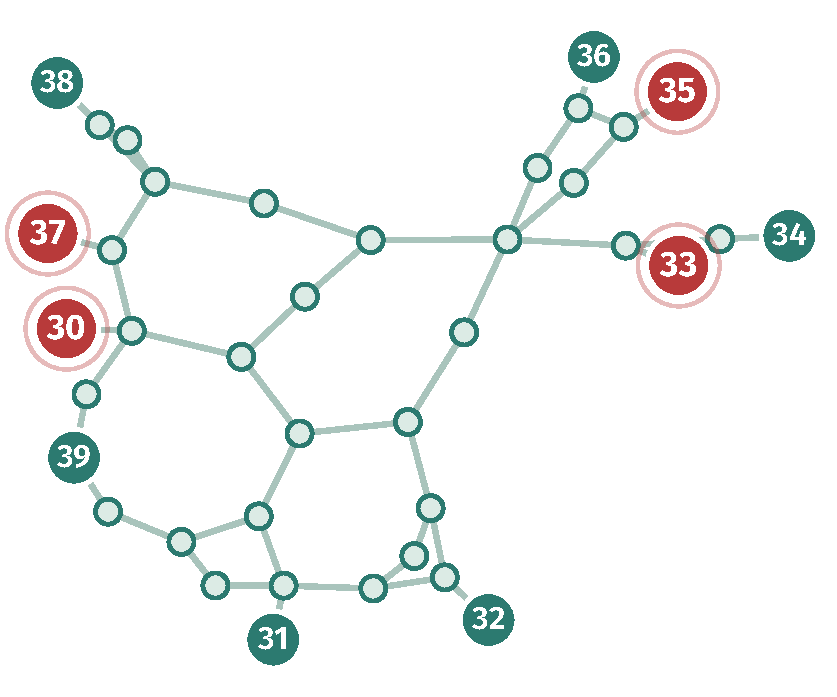
\includegraphics[width=180\PX,height=150\PY]{figures/module3/network_v2.pdf}};
  \node[anchor=north west,inner sep=0pt,text=PMuted,align=left,font=\FiraMed\fontsize{17.5pt}{19.5pt}\selectfont] at (775,322)
    {IEEE-39 grid.\ {\color{PRed}\FiraSemi Red}: the four sites\\[-1pt]of the portfolio $H_4$; teal: other SGs};

  % ---------------------------------------------------------------- B: Hasse lattice of the 16 portfolios (4-dot glyphs)
  \begin{scope}[line cap=round,line join=round]
  % node coordinates: name / x / y
  \foreach \n/\x/\y in {z/1051/303,
      a/994/272,b/1032/272,c/1070/272,d/1108/272,
      ab/978.5/241,ac/1007.5/241,ad/1036.5/241,bc/1065.5/241,bd/1094.5/241,cd/1123.5/241,
      abc/994/210,abd/1032/210,acd/1070/210,bcd/1108/210,
      e/1051/179}{\coordinate (h\n) at (\x,\y);}
  % cover relations (32 edges)
  \foreach \u/\v in {z/a,z/b,z/c,z/d, a/ab,a/ac,a/ad, b/ab,b/bc,b/bd, c/ac,c/bc,c/cd, d/ad,d/bd,d/cd,
      ab/abc,ab/abd, ac/abc,ac/acd, ad/abd,ad/acd, bc/abc,bc/bcd, bd/abd,bd/bcd, cd/acd,cd/bcd}{
    \draw[PMist,line width=1.8pt] (h\u) -- (h\v);}
  % the cliff: last step into the full set
  \foreach \u in {abc,abd,acd,bcd}{\draw[PRed,line width=2.6pt] (h\u) -- (he);}
  % glyphs: stable subsets (teal), full set (red)
  \foreach \n/\x/\y/\p/\q/\r/\s in {z/1051/303/0/0/0/0,
      a/994/272/1/0/0/0,b/1032/272/0/1/0/0,c/1070/272/0/0/1/0,d/1108/272/0/0/0/1,
      ab/978.5/241/1/1/0/0,ac/1007.5/241/1/0/1/0,ad/1036.5/241/1/0/0/1,bc/1065.5/241/0/1/1/0,bd/1094.5/241/0/1/0/1,cd/1123.5/241/0/0/1/1,
      abc/994/210/1/1/1/0,abd/1032/210/1/1/0/1,acd/1070/210/1/0/1/1,bcd/1108/210/0/1/1/1}{
    \HGlyph{\x}{\y}{\p}{\q}{\r}{\s}{8.5}{PTeal!22!PPaleGreen}{PTeal}}
  \fill[PRed!18!white,rounded corners=5pt] (1051-17,179-17) rectangle (1051+17,179+17);
  \HGlyph{1051}{179}{1}{1}{1}{1}{12.5}{PRed}{white}
  % lattice labels
  \node[anchor=west,inner sep=0pt,text=PRed,font=\FiraBold\fontsize{20pt}{20pt}\selectfont\addfontfeature{LetterSpace=3}] at (1073,176) {UNSTABLE};
  \node[anchor=west,inner sep=0pt,text=PMuted,font=\FiraMed\fontsize{17.5pt}{19pt}\selectfont] at (1068,303) {$\varnothing$ none replaced};
  \end{scope}
  \node[anchor=north west,inner sep=0pt,text=PMuted,align=left,font=\FiraMed\fontsize{17.5pt}{19.5pt}\selectfont] at (968,322)
    {Each glyph is one portfolio: filled dot\\[-1pt]= replaced site (grid 30\,33 / 35\,37).};

  % ---------------------------------------------------------------- hero: the one key number
  \HeroBox{773}{351}{1141}{397}
  \node[anchor=west,inner sep=0pt,text=PGreen,font=\FiraSemi\fontsize{22pt}{22pt}\selectfont] at (785,362) {Minimal collective blocker\ \ $H_4=\{30,33,35,37\}$};
  \node[anchor=west,inner sep=0pt,text=PNavy] at (785,383) {\fontsize{28pt}{30pt}\selectfont $\alpha_\perp(H_4)=+0.127\ \mathrm{s}^{-1}$ at $0.6223$ Hz}; % source: .../h4_crossmode_v3/claims/tx4_summary.json (alpha_P4 = 0.12700646782830968), docs/IAS26-010_ROOT_CAUSE.md (f = 0.6222796695036534 Hz)

  % ---------------------------------------------------------------- stability cliff note
  \NoteBox{773}{404}{1141}{428}{PRed}
  \node[anchor=west,inner sep=0pt,text=PRed,font=\FiraSemi\fontsize{23pt}{23pt}\selectfont] at (784,416.5) {15/15 proper subsets stable\ \textemdash\ full coalition unstable}; % source: derived/TX4_PROPER_SUBSET_CLOSURE.csv (15 rows, stable=True), claims/tx4_summary.json minimality_all_proper_stable

  % ---------------------------------------------------------------- scope
  \node[anchor=west,inner sep=0pt,text=PMuted,font=\FiraMed\fontsize{19pt}{19pt}\selectfont] at (773,440) {Canonical nominal witness, not a universal blocker.};
\end{scope}
